% THIS DOCUMENT IS FOLLOWS THE VOLERE TEMPLATE BY Suzanne Robertson and James Robertson
% ONLY THE SECTION HEADINGS ARE PROVIDED
%
% Initial draft from https://github.com/Dieblich/volere
%
% Risks are removed because they are covered by the Hazard Analysis
\documentclass[12pt]{article}

\usepackage{booktabs}
\usepackage{tabularx}
\usepackage{enumerate} 
\usepackage{hyperref}
\usepackage{enumerate}
\usepackage{graphicx}
\usepackage{float}
\usepackage{longtable}
\hypersetup{
    bookmarks=true,         % show bookmarks bar?
      colorlinks=true,      % false: boxed links; true: colored links
    linkcolor=red,          % color of internal links (change box color with linkbordercolor)
    citecolor=green,        % color of links to bibliography
    filecolor=magenta,      % color of file links
    urlcolor=cyan           % color of external links
}

\newcommand{\lips}{\textit{Insert your content here.}}

%% Comments

\usepackage{color}

\newif\ifcomments\commentstrue %displays comments
%\newif\ifcomments\commentsfalse %so that comments do not display

\ifcomments
\newcommand{\authornote}[3]{\textcolor{#1}{[#3 ---#2]}}
\newcommand{\todo}[1]{\textcolor{red}{[TODO: #1]}}
\else
\newcommand{\authornote}[3]{}
\newcommand{\todo}[1]{}
\fi

\newcommand{\wss}[1]{\authornote{blue}{SS}{#1}} 
\newcommand{\plt}[1]{\authornote{magenta}{TPLT}{#1}} %For explanation of the template
\newcommand{\an}[1]{\authornote{cyan}{Author}{#1}}

%% Common Parts

\newcommand{\progname}{Software Engineering} % PUT YOUR PROGRAM NAME HERE
\newcommand{\authname}{Team \#22, TeleHealth Insights
\\ Mitchell Weingust
\\ Parisha Nizam
\\ Promish Kandel
\\ Jasmine Sun-Hu} % AUTHOR NAMES                  

\usepackage{hyperref}
    \hypersetup{colorlinks=true, linkcolor=blue, citecolor=blue, filecolor=blue,
                urlcolor=blue, unicode=false}
    \urlstyle{same}
                                


\begin{document}

\title{Software Requirements Specification for \progname: subtitle describing software} 
\author{\authname}
\date{\today}
	
\maketitle

~\newpage

\pagenumbering{roman}

\tableofcontents

~\newpage

\section*{Revision History}

\begin{tabularx}{\textwidth}{p{2cm}p{1.5cm}p{3.5cm}X}
\toprule {\textbf{Date}} & {\textbf{Version}} & {\textbf{Contributors}} & {\textbf{Notes}}\\
\midrule
Oct 3 2024 & 1.0 & Mitchell Weingust, Parisha Nizam & Added Functional Requirements 9.1, 9.2, 9.3 \\
Oct 3 2024 & 1.1 & Promish Kandel, Jasmine Sun-Hu & Added Functional Requirements 9.4,9.5,9.6, and sections 1,3,5\\
Oct 4 2024 & 1.2 & Mitchell Weingust, Parisha Nizam & Added Non Functional Requirements 11, 13, 15, 17\\
Oct 4 2024 & 1.3 & Jasmine Sun-Hu & Added Nonfunctional Requirements 10,14,16\\
Oct 5 2024 & 1.4 & Promish Kandel & Added Nonfunctional Requirements 12\\
Oct 6 2024 & 1.5 & Mitchell Weingust, Parisha Nizam & Added Sections 2, 4\\
Oct 9 2024 & 1.6 & Mitchell Weingust & Added Sections 8, 18\\
\bottomrule
\end{tabularx}

~\\

~\newpage
\section{Purpose of the Project}
\subsection{User Business}
\hspace{2em}The project being outlined in this document is an at-home bilingual speech 
assessment system with video and audio analysis features. The system is designed 
to provide clear guidance to parents when administering the assessment to their 
children, in an environment where speech-language pathologists (SLPs) are 
unavailable. By streamlining the assessment process, the project aims to provide a 
convenient and comprehensive solution for SLPs to assess and support their patients'
speech and language development remotely. 
\subsection{Goals of the Project}
\begin{itemize}
  \item[1.2.1] \textbf{Intuitive Parent Interface:}  
  The system must provide an intuitive interface that helps parents administer 
  language assessments effectively. It should be easy to navigate with clear and 
  meaningful symbols, and it must provide real-time feedback to ensure parents are 
  aware their interactions are being processed throughout the assessment.

  \item[1.2.2] \textbf{Engaging Child Interaction:}  
  The system must feature an engaging interface for children to keep them attentive 
  during the assessment. The design should be simple yet visually appealing, using 
  colors and images to attract the child’s attention to the questions and selections,
  ensuring that children remain engaged throughout the assessment.

  \item[1.2.3] \textbf{Reliable Assessment Data for SLPs:}  
  The system must provide reliable and accurate assessment data for speech-language 
  pathologists (SLPs) by capturing additional contextual data. This includes 
  identifying background interference, signs of bias, and potential test 
  complications. The system should also filter out noise and detect multiple users 
  to prevent external guidance from affecting the assessment results.

  \item[1.2.4] \textbf{Data Security:}  
  The system must ensure that all sensitive health and personal data is securely 
  stored and accessed. It should implement a strong security protocol to securely 
  store, retrieve, and manage sensitive data, ensuring the privacy and confidentiality
  of the users.

  \item[1.2.5] \textbf{Cross-Platform Compatibility:}  
  The system must provide cross-platform compatibility, ensuring that it functions 
  seamlessly across different devices and screen sizes. It should be accessible to 
  both parents and children, rendering correctly on all screen formats, whether on 
  phones, tablets, or desktops.
\end{itemize}

\section{Stakeholders}
\subsection{Client}
This project's client is Researcher, Clinician Assistant, Professor at the University of Southern California, Dr. Yao Du.
\subsection{Customer}
This project's customers are Clinicians (SLPs) who work with children that have speech difficulties.
\subsection{Other Stakeholders}
Another stakeholder is this project's supervisor, Dr. Irene Ye Yuan, Assistant Professor in the Department of Computing and Software at McMaster University.

\subsection{Hands-On Users of the Project}
Hands-on users for this project include the parents of children that have speech difficulties, as well as the children themselves, who need to take language assessments.
\subsection{Personas}
\textbf{User Profile:}\\
Name: Paul Blart\\
Age: 42\\
Job: Mall Cop\\
Personality Traits: Caring, Strict, Empathetic, Impatient, Stubborn\\

\textbf{Key Task Goals:}
\begin{itemize}
  \item Convenient access to healthcare technology for his family.
  \item Use a system that is easy for both him and his child to learn and use.
  \item Wants a system that is available for him to use at any time, as his job doesn't usually allow him to schedule in-person assessments easily.
  \item Cares about his family's safety and security, so he wants a system that will keep their healthcare and personal information confidential.  
\end{itemize}

\textbf{Motivations/Frustrations:}
\begin{itemize}
  \item Paul is motivated by caring for his child, and wants the best support for them.
  \item Paul is encouraged to find a system that his child can easily navigate, so it does not stress them out or make their lives more difficult.
  \item Paul is frustrated by systems that take too long to load.
  \item Paul is frustrated by systems that are not easy to use, as he often has to dedicate long periods of time to learn new technology.
  \item Paul doesn't like changing his routine, so he wants to find a system that works for him, and stick with it.
  \item Paul is motivated to find a system that will best help his child so he can see how their language understanding improves over time.
\end{itemize}

\textbf{Quote:}\\
'Man, technology is so hard! I love my kid, but I am so busy. My kid doesn't like going in person to speak with clinicians. I need a solution that will make them feel more comfortable. I wish there was a way to track their progress, so I can see how they're improving.'\\

\subsection{Priorities Assigned to Users}
\begin{enumerate}
  \item Parents
  \item Children (who take learning assessments)
  \item SLPs
  \item Researcher (Dr. Yao Du)
  \item Supervisor (Dr. Irene Ye Yuan)
\end{enumerate}
\subsection{User Participation}
\begin{itemize}
  \item Parents
  \subitem{No input necessary.}
  \item Children (who take learning assessments)
  \subitem{No input necessary.}
  \item SLPs
  \subitem{No input necessary.}
  \item Researcher (Dr. Yao Du)
  \subitem{Occassional input, communication is managed through the project's supervisor.}
  \item Supervisor (Dr. Irene Ye Yuan)
  \subitem{Frequent input, with minimum weekly checkins to ensure the project is within scope and on-track.}
\end{itemize}

\subsection{Maintenance Users and Service Technicians}
N/A\\

\section{Mandated Constraints}
\subsection{Solution Constraints}
\begin{itemize}
  \item[3.1.1] The platform must be accessible as a website to provide ease of access to users without requiring special software installations.
  \item[3.1.2] The platform must adhere to HIPAA or relevant data protection regulations to ensure patient data privacy and security.
  \item[3.1.3] Access to the platform must be restricted to authorized users, with secure authentication processes in place.
  \item[3.1.4] The system must be capable of scaling to accommodate an increasing number of users and growing data storage needs as the client expands.
  \item[3.1.5] The platform must support assessment sessions of up to at least 30 minutes to align with standard telehealth consultation times.
  \item[3.1.6] The platform must support adaptable video and audio quality based on internet bandwidth, ensuring clarity and reliability during assessments.
  \item[3.1.7] The platform must comply with WCAG 2.1 accessibility standards, making it accessible to users with varying needs.
  \item[3.1.8] Patient records must be retained for a minimum of 7 years from the last visit or at least 1 year after the patient turns 18, whichever is 
  longer, in accordance with California law.
\end{itemize}
\subsection{Implementation Environment of the Current System}
\begin{itemize}
  \item[3.2.1] The platform’s hosting environment must meet HIPAA-compliance standards to ensure data security.
  \item[3.2.2] The development framework must support scalable, secure, and efficient web application development, compatible with existing technical 
  infrastructure.
\end{itemize}
\subsection{Partner or Collaborative Applications}
\begin{itemize}
  \item[3.3.1] The platform must be capable of exporting data as an Excel file, allowing for easy sharing, analysis, and compatibility with other systems
  that clinicians may use for data processing.
\end{itemize}
\subsection{Off-the-Shelf Software}
\begin{itemize}
  \item[3.4.1] \color{red} There are no mandated off-the-shelf software constraints. \color{black}
\end{itemize}
\subsection{Anticipated Workplace Environment}
\begin{itemize}
  \item[3.5.1] The platform must be compatible across a range of devices, including desktops, tablets, and mobile phones.
\end{itemize}
\subsection{Schedule Constraints}
\begin{itemize}
  \item[3.6.1] The proof-of-concept shall be complete and demonstrated between Nov. 11-22, 2024.
  \item[3.6.2] Revision 0 of the project shall be complete and demonstrated between February 3-14, 2025.
  \item[3.6.3] The final product shall be complete and demonstrated between March 24-30, 2025.
\end{itemize}
\subsection{Budget Constraints}
\begin{itemize}
  \item[3.7.1] The project budget must not exceed \$750 CAD. 
\end{itemize}
\subsection{Enterprise Constraints}
\begin{itemize}
  \item[3.8.1] \color{red} There are no mandated enterprise constraints. \color{black}
\end{itemize}

\section{Naming Conventions and Terminology}
\subsection{Glossary of All Terms, Including Acronyms, Used by Stakeholders
involved in the Project}

\begin{tabularx}{\textwidth}{p{2cm}X}
  \toprule {\textbf{Terms}} & {\textbf{Definition}}\\
  \midrule
  SLP & Speech Language Pathologist\\
  HIPAA & Health Insurance Portability and Accountability Act\\
  WCAG & Web Content Accessibility Guidelines\\
  \bottomrule
\end{tabularx}

\section{Relevant Facts And Assumptions}
\subsection{Relevant Facts}
\begin{itemize}
  \item[5.1.1] The project is subject to healthcare privacy laws like HIPAA, ensuring that patient data is securely stored and managed.
  \item[5.1.2] The client has requested a web-based platform, indicating a preference for accessibility without the need for specialized 
  software installations.
  \item[5.1.3] The platform will have two primary user roles. The clinicians who perform assessments and review results and the parents who 
  administer the assessment to their children who are the patients.
\end{itemize}
\subsection{Business Rules}
\begin{itemize}
  \item[5.2.1] Only authorized users (clinicians) can access patient data.
  \item[5.2.2] Patient records must be retained for at least 7 years from the last visit, or 1 year after the patient turns 18, whichever is longer, 
  to comply with California state law.
  \item[5.2.3] The platform must comply with WCAG 2.1 to ensure it is accessible to users with disabilities.
  \item[5.2.4] All patient data must be encrypted both in transit and at rest to maintain confidentiality and meet regulatory standards.
  \item[5.2.5] The platform must generate reports based on assessment data, which can be reviewed and stored within the system 
  \item[5.2.6] Video and audio recordings must automatically adjust to optimize based on internet bandwidth, ensuring quality without excessive 
  buffering or latency.
\end{itemize}
\subsection{Assumptions}
\begin{itemize}
  \item[5.3.1] All users of the system have reliable internet connections that can support telehealth video sessions.
  \item[5.3.2] All patient data will be stored on servers located in regions that comply with healthcare data residency regulations.
  \item[5.3.3] The platform is assumed to be accessible from various devices (desktops, tablets, mobile phones), though it may perform optimally on 
  desktops.
  \item[5.3.4] Assessments will not exceed 30 minutes per session to fit standard telehealth consultation times.
  \item[5.3.5] It is assumed that users (both clinicians and patients) have a basic level of comfort with using web applications and online 
  communication tools.
  \item[5.3.6] The platform may need to accommodate additional users and storage demands as the client scales its telehealth services over time.
\end{itemize}

\section{The Scope of the Work}
\subsection{The Current Situation}
\lips
\subsection{The Context of the Work}
\lips
\subsection{Work Partitioning}
\lips
\subsection{Specifying a Business Use Case (BUC)}
\lips

\section{Business Data Model and Data Dictionary}
\subsection{Business Data Model}
\lips
\subsection{Data Dictionary}
\lips

\section{The Scope of the Product}
\subsection{Product Boundary}
\begin{figure}[H]
  \centering
  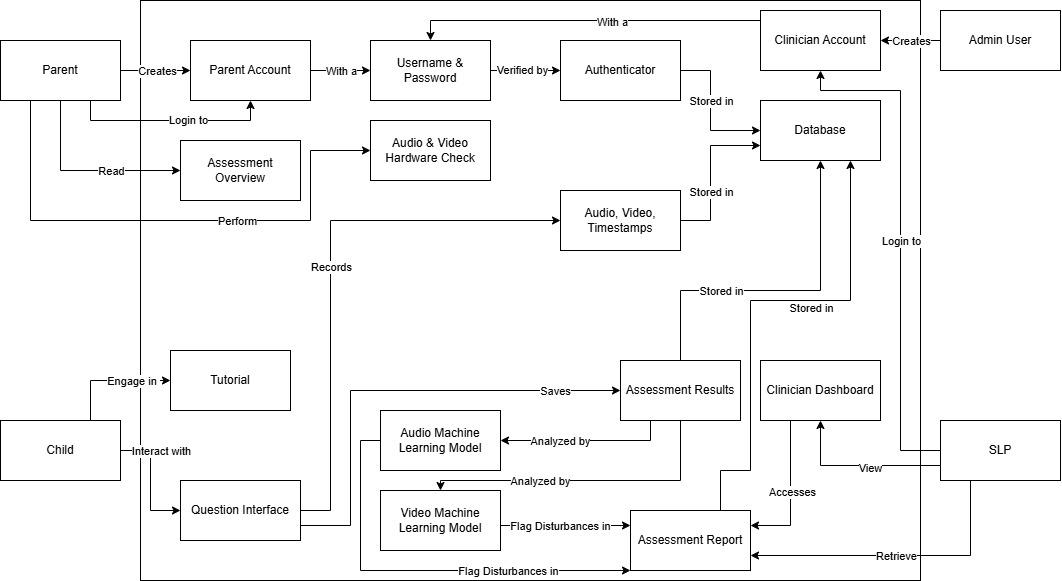
\includegraphics[scale=0.45]{images/BoundaryDiagram.jpg}
  \caption{Boundary Diagram}
\end{figure}
\begin{figure}[H]
  \centering
  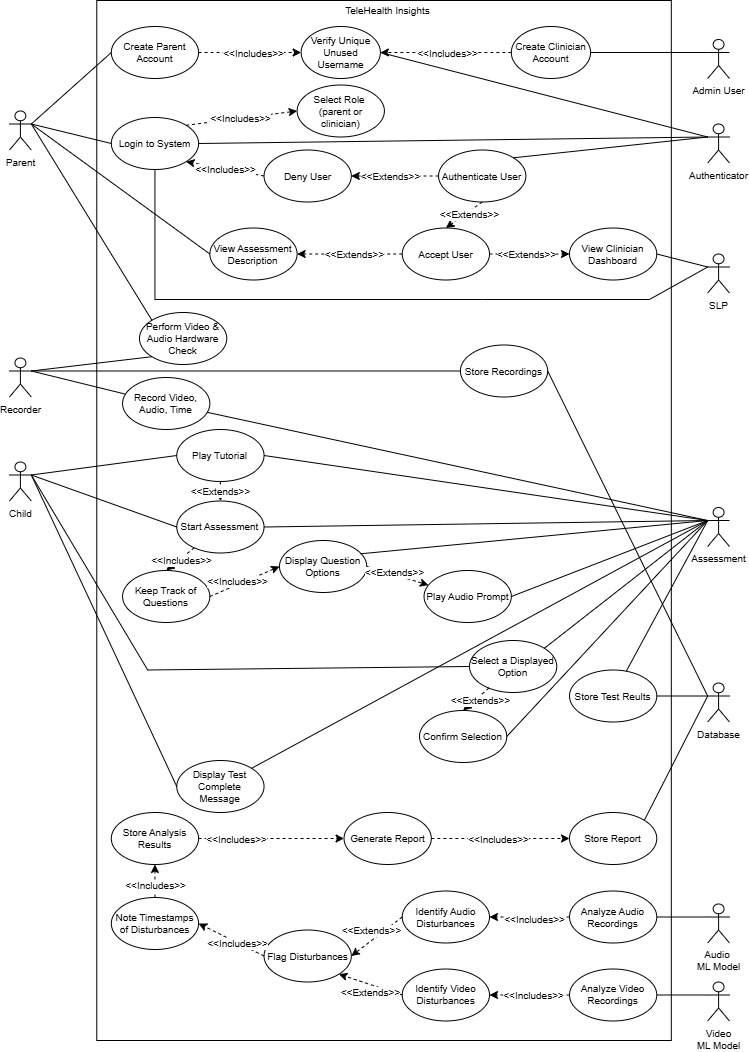
\includegraphics[scale=0.5]{images/UseCaseDiagram.jpg}
  \caption{User Case Diagram}
\end{figure}
\subsection{Product Use Case Table}
\begin{longtable}{|p{2cm}|p{3.2cm}|p{3.2cm}|p{3cm}|p{3cm}|}
  \toprule {\textbf{PUC No.}} & {\textbf{PUC Name}} & {\textbf{Actor(s)}} & {\textbf{Input(s)}} & {\textbf{Output(s)}} \\
  \midrule
  PUC-01 & Create Parent Account & Parent & Username \& Password & \\
  \hline
  PUC-02 & Verify Unique Unused Username & Parent \& Authenticator & Username & Account Created or Failure Message\\
  \hline
  PUC-03 & Create Clinician Account & Admin User \& Authenticator & Username \& Password & \\
  \hline
  PUC-04 & Login to System & Parent \& Authenticator \& SLP & Username \& Password & \\
  \hline
  PUC-05 & Select Role & Parent \& SLP & Role Selection & \\
  \hline
  PUC-06 & Deny User & Parent \& Authenticator \& SLP & & Login failure message\\
  \hline
  PUC-07 & Authenticate User & Authenticator & Username \& Password & \\
  \hline
  PUC-08 & Accept User & Authenticator & & Go to View Assessment Description or View Clinician Dashboard\\
  \hline
  PUC-09 & View Assessment Description & Parent & & Display Assessment Description\\
  \hline
  PUC-10 & View Clinician Dashboard & SLP & & Display Clinician Dashboard\\
  \hline
  PUC-11 & Perform Video \& Audio Hardware Check & Parent \& Recorder & Sound Input \& Video Input & Confirmation Message or Repeat Procedure\\
  \hline
  PUC-12 & Store Recordings & Recorder \& Database & Audio Recordings \& Video Recordings & \\
  \hline
  PUC-13 & Record Video, Audio, Time & Recorder \& Assessment & Video Recordings \& Audio Recordings \& Timer & \\
  \hline
  PUC-14 & Play Tutorial & Child \& Assessment & Click Play Tutorial Button & Plays Tutorial\\
  \hline
  PUC-15 & Start Assessment & Child \& Authenticator & Click Start Assessment Button & Go to First Question\\
  \hline
  PUC-16 & Keep Track of Questions & Assessment & Click Confirm Selection& Question Number\\
  \hline
  PUC-17 & Display Question Options & Assessment & & Display Options\\
  \hline
  PUC-18 & Play Audio Prompt & Assessment & & Plays Audio\\
  \hline
  PUC-19 & Retrieve Assessment Results & Assessment \& Database & Complete Assessment &\\
  \hline
  PUC-20 & Select a Displayed Option & Child \& Assessment & Select Option & Highlight Option\\
  \hline
  PUC-21 & Confirm Selection & Child \& Assessment & Select Confirm Selection & Go to Next Question or Test Complete\\
  \hline
  PUC-22 & Display Test Complete Message & Child \& Assessment & Select final Confirm Selection & Display Message\\
  \hline
  PUC-23 & Store Test Results & Assessment \& Database & Test Results & Store Results\\
  \hline
  PUC-24 & Analyze Audio Recordings & Audio ML Model & Audio Recording & Analyzed Recording Data\\
  \hline
  PUC-25 & Identify Audio Disturbances & Audio ML Model & Analyzed Recording Data & List of disturbances\\
  \hline
  PUC-26 & Analyze Video Disturbances & Video ML Model & Video Recording & Analyzed Recording Data\\
  \hline
  PUC-27 & Identify Video Disturbances & Video ML Model & Analyzed Recording Data & List of disturbances\\
  \hline
  PUC-28 & Flag Disturbances & Audio ML Model \& Video ML Model & List of disturbances & Timestamp Markers\\
  \hline
  PUC-29 & Note Timestamp of Disturbance & Audio ML Model \& Video ML Model & Timestampe Markers & Report Data\\
  \hline
  PUC-30 & Store Analysis Results & Audio ML Model \& Video ML Model \& Database & Report Data & Analaysis Results\\
  \hline
  PUC-31 & Generate Report & Database & Analysis Results & Assessment Report\\
  \hline
  PUC-32 & Store Report & Database & Assessment Report & Store Report\\
  \bottomrule
\end{longtable}
\subsection{Individual Product Use Cases (PUC's)}
\begin{enumerate}[{PUC-}01. ]
  \item Create Parent Account\\
  \textbf{Precondition: }None\\
  \textbf{Trigger: }Parent selects 'Create Account'\\
  \textbf{Outcome: }Parent is brought to screen to Create Account with their information\\
  \textbf{Postcondition: } Parent's account creation is verified by authenticator\\
\end{enumerate}

\begin{enumerate}[{PUC-}02. ]
  \item Verify Unique Unused Username\\
  \textbf{Precondition: }Parent or Admin user creates a new account\\
  \textbf{Trigger: }User attempts to complete creating their account\\
  \textbf{Outcome: }User is logged into their newly created account\\
  \textbf{Postcondition: }User's account is created, or, User needs to select a unique username\\
\end{enumerate}

\begin{enumerate}[{PUC-}03. ]
  \item Create Clinician Account\\
  \textbf{Precondition: }Clinician goes to their admin user to request account creation\\
  \textbf{Trigger: }Admin user creates a new clincian account\\
  \textbf{Outcome: }\\
  \textbf{Postcondition: }Clinician's account creation is verified by authenticator\\
\end{enumerate}

\begin{enumerate}[{PUC-}04. ]
  \item Login to System\\
  \textbf{Precondition: }User intentionally goes to login screen, or, authenticator denies user\\
  \textbf{Trigger: }User selects login button from home screen, or, user logs in with incorrect credentials\\
  \textbf{Outcome: }\\
  \textbf{Postcondition: }User enters into system logged into their account\\
\end{enumerate}

\begin{enumerate}[{PUC-}05. ]
  \item Select Role\\
  \textbf{Precondition: }User is on login screen\\
  \textbf{Trigger: }User selects their role (choosing between parent or clinician)\\
  \textbf{Outcome: }\\
  \textbf{Postcondition: }Role is selected for relevant system access\\
\end{enumerate}

\begin{enumerate}[{PUC-}06. ]
  \item Deny User\\
  \textbf{Precondition: }Authenticator could not authenticate user with their credentials\\
  \textbf{Trigger: }User entered incorrect credentials for their account\\
  \textbf{Outcome: }User is denied entry into their account\\
  \textbf{Postcondition: }User is returned to the login screen\\
\end{enumerate}

\begin{enumerate}[{PUC-}07. ]
  \item Authenticate User\\
  \textbf{Precondition: }User attempted to login to their account\\
  \textbf{Trigger: }User entered their login information on login screen\\
  \textbf{Outcome: }Authenticator verifies against account details stored in system\\
  \textbf{Postcondition: }User is accepted or denied\\
\end{enumerate}

\begin{enumerate}[{PUC-}08. ]
  \item Accept User\\
  \textbf{Precondition: }User login information has been verified by the Authenticator\\
  \textbf{Trigger: }User successfully inputs correct account information\\
  \textbf{Outcome: }User is logged into their account in the system\\
  \textbf{Postcondition: }
  \begin{enumerate}
    \item If user is a clinician, user is brought to clinician dashboard
    \item If user is a parent, user is brought to view assessment description and details
  \end{enumerate}

\end{enumerate}

\begin{enumerate}[{PUC-}09. ]
  \item View Assessment Description\\
  \textbf{Precondition: }User successfully logs into the system as a parent\\
  \textbf{Trigger: }User is verified by the authenticator upon logging in\\
  \textbf{Outcome: }\\
  \textbf{Postcondition: }Assessment description details are displayed on screen\\
\end{enumerate}

\begin{enumerate}[{PUC-}10. ]
  \item View Clinician Dashboard\\
  \textbf{Precondition: }User successfully logs into the system as a clincian\\
  \textbf{Trigger: }User is verified by the authenticator upon logging in\\
  \textbf{Outcome: }\\
  \textbf{Postcondition: }Clinician dashboard is displayed on screen\\
\end{enumerate}

\begin{enumerate}[{PUC-}11. ]
  \item Perform Video \& Audio Hardware Check\\
  \textbf{Precondition: }Parent read over the assessment details\\
  \textbf{Trigger: }Parent selects setup video and audio hardware check\\
  \textbf{Outcome: }Parent performs video and audio hardware check\\
  \textbf{Postcondition: }Tutorial is displayed on screen for child to engage with\\
\end{enumerate}

\begin{enumerate}[{PUC-}12. ]
  \item Store Recordings\\
  \textbf{Precondition: }User has completed the assessment\\
  \textbf{Trigger: }User has confirmed their selection on the final question of the assessment\\
  \textbf{Outcome: }Recording is stopped\\
  \textbf{Postcondition: }Recording is saved in the database\\
\end{enumerate}

\begin{enumerate}[{PUC-}13. ]
  \item Record Video, Audio, Time\\
  \textbf{Precondition: }User has completed the video and hardware check\\
  \textbf{Trigger: }User confirms start of the assessment\\
  \textbf{Outcome: }Recording has started\\
  \textbf{Postcondition: }Record the user's video, audio, and time\\
\end{enumerate}

\begin{enumerate}[{PUC-}14. ]
  \item Play Tutorial\\
  \textbf{Precondition: }Parent has completed video and audio hardware check\\
  \textbf{Trigger: }Child confirms starting the tutorial\\
  \textbf{Outcome: }\\
  \textbf{Postcondition: }Tutorial plays on-screen\\
\end{enumerate}

\begin{enumerate}[{PUC-}15. ]
  \item Start Assessment\\
  \textbf{Precondition: }User has completed watching the tutorial\\
  \textbf{Trigger: }User confirms selection of starting assessment\\
  \textbf{Outcome: }Assessment begins\\
  \textbf{Postcondition: }Go to first question\\
\end{enumerate}

\begin{enumerate}[{PUC-}16. ]
  \item Keep Track of Questions\\
  \textbf{Precondition: }Assessment has started\\
  \textbf{Trigger: }Confirming selection after choosing from a question's options\\
  \textbf{Outcome: }\\
  \textbf{Postcondition: }Displayed question information is updated\\
\end{enumerate}

\begin{enumerate}[{PUC-}17. ]
  \item Display Question Options\\
  \textbf{Precondition: }User started the assessment\\
  \textbf{Trigger: }A new question is displayed on screen\\
  \textbf{Outcome: }\\
  \textbf{Postcondition: }Corresponding question options are displayed on screen\\
\end{enumerate}

\begin{enumerate}[{PUC-}18. ]
  \item Play Audio Prompt\\
  \textbf{Precondition: }User is on a question page\\
  \textbf{Trigger: }Question options are displayed\\
  \textbf{Outcome: }\\
  \textbf{Postcondition: }Audio prompt is played\\
\end{enumerate}

\begin{enumerate}[{PUC-}19. ]
  \item Retrieve Assessment Results\\
  \textbf{Precondition: }Assessment is complete\\
  \textbf{Trigger: }User has confirmed their selection on the final question\\
  \textbf{Outcome: }\\
  \textbf{Postcondition: }Assessment results are stored in the database\\
\end{enumerate}

\begin{enumerate}[{PUC-}20. ]
  \item Select a Displayed Option\\
  \textbf{Precondition: }Question's corresponding audio has played for the user\\
  \textbf{Trigger: }User selects amongst the options displayed\\
  \textbf{Outcome: }\\
  \textbf{Postcondition: }Indicate to the user, visually, which option they selected\\
\end{enumerate}

\begin{enumerate}[{PUC-}21. ]
  \item Confirm Selection\\
  \textbf{Precondition: }User selected an option\\
  \textbf{Trigger: }User selects 'Confirm Selection'\\
  \textbf{Outcome: }User's chosen option is confirmed and saved\\
  \textbf{Postcondition: }User goes to next question, or, if this is the final question, display test completion message\\
\end{enumerate}

\begin{enumerate}[{PUC-}22. ]
  \item Display Test Complete Message\\
  \textbf{Precondition: }User is on the final question\\
  \textbf{Trigger: }User confirmed their option selection\\
  \textbf{Outcome: }\\
  \textbf{Postcondition: }Test complete message is displayed\\
\end{enumerate}

\begin{enumerate}[{PUC-}23. ]
  \item Store Test Results\\
  \textbf{Precondition: }Test is complete\\
  \textbf{Trigger: }Test complete message is displayed\\
  \textbf{Outcome: }\\
  \textbf{Postcondition: }Test results are stored in the database\\
\end{enumerate}

\begin{enumerate}[{PUC-}24. ]
  \item Analyze Audio Recordings\\
  \textbf{Precondition: }Audio recordings are stored in the database\\
  \textbf{Trigger: }\\
  \textbf{Outcome: }Audio recordings are processed by the audio machine learning model\\
  \textbf{Postcondition: }\\
\end{enumerate}

\begin{enumerate}[{PUC-}25. ]
  \item Identify Audio Disturbances\\
  \textbf{Precondition: }Audio recordings have been processed by the audio machine learning model\\
  \textbf{Trigger: }\\
  \textbf{Outcome: }\\
  \textbf{Postcondition: }Audio disturbances are identified\\
\end{enumerate}

\begin{enumerate}[{PUC-}26. ]
  \item Analyze Video Disturbances\\
  \textbf{Precondition: }Video recordings are stored in the database\\
  \textbf{Trigger: }\\
  \textbf{Outcome: }\\
  \textbf{Postcondition: }Video recordings are processed by the video machine learning model\\
\end{enumerate}

\begin{enumerate}[{PUC-}27. ]
  \item Identify Video Disturbances\\
  \textbf{Precondition: }Video recordings have been processed by the video machine learning model\\
  \textbf{Trigger: }\\
  \textbf{Outcome: }\\
  \textbf{Postcondition: }Video disturbances are identified\\
\end{enumerate}

\begin{enumerate}[{PUC-}28. ]
  \item Flag Disturbances\\
  \textbf{Precondition: }Audio and Video disturbances have been identified.\\
  \textbf{Trigger: }\\
  \textbf{Outcome: }Disturbances are flagged for the clinician to review\\
  \textbf{Postcondition: }Flagged disturbances are noted to find the corresponding timestamp of the occurrence\\
\end{enumerate}

\begin{enumerate}[{PUC-}29. ]
  \item Note Timestamp of Disturbance\\
  \textbf{Precondition: }Flagged disturbances have been recorded\\
  \textbf{Trigger: }\\
  \textbf{Outcome: }Timestamps to be synced with the video and audio recordings are noted\\
  \textbf{Postcondition: }Timestamps of flags are stored in the analysis results\\
\end{enumerate}

\begin{enumerate}[{PUC-}30. ]
  \item Store Analysis Results\\
  \textbf{Precondition: }Disturbances have been identified, flagged, and corresponding timestamps have been recorded\\
  \textbf{Trigger: }\\
  \textbf{Outcome: }\\
  \textbf{Postcondition: }Analysis results are stored as data for the clinician report\\
\end{enumerate}

\begin{enumerate}[{PUC-}31. ]
  \item Generate Report\\
  \textbf{Precondition: }Analysis results have been stored\\
  \textbf{Trigger: }\\
  \textbf{Outcome: }\\
  \textbf{Postcondition: }Clincian report is generated with data from the assessment analysis\\
\end{enumerate}

\begin{enumerate}[{PUC-}32. ]
  \item Store Report\\
  \textbf{Precondition: }Clinician report is generated\\
  \textbf{Trigger: }\\
  \textbf{Outcome: }Report is available to be viewed and accessed by the clinician\\
  \textbf{Postcondition: }Clinician report is stored in the database\\
\end{enumerate}


\section{Functional Requirements}

\subsection{Authentication}
\begin{enumerate}[{FR-A}1. ]
  \item The system shall allow a user to choose between a Parent or Clinician account prior to logging in.\\
  \textbf{Rationale: }Users must be associated with the correct permissions determined by their role, which includes the level of information they have access to.\\
  \textbf{Fit criterion: }Users must be able to directly select their account type prior to logging in. 
\end{enumerate}
\begin{enumerate}[{FR-A}2. ]
  \item The system shall allow a user to create a parent account with a unique username which does not exist in the database.\\
  \textbf{Rationale: }Users must be able to create a unique account for parents to login for the assessment.\\
  \textbf{Fit criterion: }Users cannot create accounts with usernames that already exist in the database.
\end{enumerate}
\begin{enumerate}[{FR-A}3. ]
  \item The system shall allow a user with admin privilege to create a clinician account with a unique username which does not exist in the database.\\
  \textbf{Rationale: }Admin-Users must be able to create a unique account for clinicians to login to view assessment results. Clinicians need to be approved by Admin-Users to have a clinician account.\\
  \textbf{Fit criterion: }Users cannot create clinician accounts, without admin access, with usernames that already exist in the database. 
\end{enumerate}
\begin{enumerate}[{FR-A}4. ]
  \item The system shall allow a user with a unique username to login with their corresponding password.\\
  \textbf{Rationale: }Users must be able to login to their account to restrict others from accessing their assessment or assessment results.\\
  \textbf{Fit criterion: }Users must be able to provide the corresponding password to their unique username to login and successfully enter the system. 
\end{enumerate}
\begin{enumerate}[{FR-A}5. ]
  \item The system shall allow a user to logout.\\
  \textbf{Rationale: }Users must be able to logout of their account to restrict others from accessing their information.\\
  \textbf{Fit criterion: }Users must be able to logout and successfully exit the system.
\end{enumerate}

\subsection{System Setup}
\begin{enumerate}[{FR-SS}1. ]
  \item The system shall allow a user to view information about the assessment.\\
  \textbf{Rationale: }Users must be informed about relevant assessment information prior to starting the hardware checks.\\
  \textbf{Fit criterion: }Users must be able to view information about the assessment upon logging in.
\end{enumerate}
\begin{enumerate}[{FR-SS}2. ]
  \item The system shall allow a user to perform an audio hardware check.\\
  \textbf{Rationale: }Users must be able to perform an audio equipment check to ensure their input and output audio devices are functioning.\\
  \textbf{Fit criterion: }Users must be able to verify their audio devices are functioning with the system.
\end{enumerate}
\begin{enumerate}[{FR-SS}3. ]
  \item The system shall allow a user to perform a video hardware check.\\
  \textbf{Rationale: }Users must be able to perform an video equipment check to ensure their video capturing device is functioning.\\
  \textbf{Fit criterion: }Users must be able to verify their video capturing device is functioning with the system.  
\end{enumerate}
\begin{enumerate}[{FR-SS}4. ]
  \item The system shall provide a tutorial for a user to learn the assessment process.\\
  \textbf{Rationale: }Users must be able to walkthrough a tutorial to understand how to properly complete the assessment.\\
  \textbf{Fit criterion: }Users must be brought to the tutorial upon completing the audio and video hardware checks.  
\end{enumerate}
\begin{enumerate}[{FR-SS}5. ]
  \item The system shall allow a user to start an assessment.\\
  \textbf{Rationale: }Users must be able to decide when they start an assessment.\\
  \textbf{Fit criterion: }Users must be brought to the first assessment question upon starting the assessment.  
\end{enumerate}

\subsection{Assessment Interface}
\begin{enumerate}[{FR-AI}1. ]
  \item The system shall record user's audio and video upon starting the assessment.\\
  \textbf{Rationale: }The system must be able to collect audio and video recordings for future analysis.\\
  \textbf{Fit criterion: }The system must indicate to the user that audio and video recordings are ongoing.  
\end{enumerate}
\begin{enumerate}[{FR-AI}2. ]
  \item The system shall play audio prompts at the beginning of each question.\\
  \textbf{Rationale: }The system must be able to play the respective question's audio to answer the given question.\\
  \textbf{Fit criterion: }The system must successfully play the respective question's audio upon entering a new question.
\end{enumerate}
\begin{enumerate}[{FR-AI}3. ]
  \item The system shall display a question's options for a user to select.\\
  \textbf{Rationale: }Users must be able to provide a response to the question's audio for future analysis.\\
  \textbf{Fit criterion: }The system must display the question's respective options upon starting a new question.
\end{enumerate}
\begin{enumerate}[{FR-AI}4. ]
  \item The system shall allow a user to select one of the displayed options.\\
  \textbf{Rationale: }Users must be able to select their best option to answer the question.\\
  \textbf{Fit criterion: }The system must indicate to the user their selected response.
\end{enumerate}
\begin{enumerate}[{FR-AI}5. ]
  \item The system shall allow a user to confirm their selection.\\
  \textbf{Rationale: }Users must be able to confirm their selection to proceed to the next stage.\\
  \textbf{Fit criterion: }Users must be brought to the next stage upon confirming their selection.
\end{enumerate}
\begin{enumerate}[{FR-AI}6. ]
  \item The system shall keep track of the user's current question.\\
  \textbf{Rationale: }The system must be able to keep track of the time the user enters and exits each question, to synchronize with the audio and video recordings.\\
  \textbf{Fit criterion: }The system must store the user's timestamps upon completing each question.
\end{enumerate}
\begin{enumerate}[{FR-AI}7. ]
  \item The system shall inform the user about the assessment's completion.\\
  \textbf{Rationale: }The system must inform the user of the test's completion to indicate they can exit the system.\\
  \textbf{Fit criterion: }The user must be informed about the test's completion upon confirming the selection of the final question.
\end{enumerate}

\subsection{Data Collection and Storage}
\begin{enumerate}[{FR-DSC}1. ]
  \item The database shall be able to store multimedia files including video, audio, and structured data files for each session.\\
  \textit{Insert formal Specification}\\
  \textbf{Rationale: }These file types are necessary to capture the full scope of the speech-language assessment, 
  including patient responses and the structured data associated with each session (e.g., flagged occurrences, 
  timestamps).\\
  \textbf{Fit criterion: }The system must successfully store and retrieve at least 1GB of video, audio, and JSON 
  data per session without data corruption.
\end{enumerate}
\begin{enumerate}[{FR-DSC}2. ]
  \item The database shall store the video, audio, flagged occurrences (e.g., errors or critical moments
  during the assessment), and timestamps for each question during the assessment.\\
 \textit{Insert formal Specification}\\
 \textbf{Rationale: }Storing flagged occurrences and timestamps lets clinicians perform detailed analysis 
 of patient responses and enables them to review specific moments of interest efficiently.\\
 \textbf{Fit criterion: }The database shall include video and audio files for 100 percent of assessment sessions,
  and each recording must have flagged occurrences and timestamps associated with every question asked, 
  retrievable via query.
\end{enumerate}
\begin{enumerate}[{FR-DSC}3. ]
  \item The system shall not store any personally identifiable textual information (e.g., patient name, address, 
  or medical record number) in the database.\\
  \textit{Insert formal Specification}\\
  \textbf{Rationale: }To maintain privacy and ensure compliance with data protection regulations such as HIPAA, 
  identifying textual information must be excluded from storage in the database.\\
  \textbf{Fit criterion: }An automated process shall verify and confirm that 100\% of records in the database 
  accessible by clinicians are anonymized and contain no identifying textual information.
\end{enumerate}
\begin{enumerate}[{FR-DSC}4. ]
  \item The database shall group all stored data by a unique user identifier to ensure data can be linked to 
  individual users.\\
  \textit{Insert formal Specification}\\
  \textbf{Rationale: }Using a unique user identifier allows for data organization and retrieval by patient without 
  compromising patient privacy, supporting the requirement for anonymized data storage.\\
  \textbf{Fit criterion: }The system must assign a unique identifier to every user and confirm through testing 
  that 100\% of session data is properly grouped and retrievable under that identifier, with no unassociated 
  data.
\end{enumerate}

\subsection{Video and Audio Data Analysis}
\begin{enumerate}[{FR-VADA}4. ]
  \item The analysis model shall have access to the video and audio recordings of each session.\\
  \textit{Insert formal Specification}\\
  \textbf{Rationale: }The data contains essential visual and auditory information that can help clinicians 
  efficiently assess any speech-related disturbances and non-verbal cues.\\
  \textbf{Fit criterion: }The model must successfully retrieve and process video data from 100\% of 
  completed assessment sessions without encountering data access errors.
\end{enumerate}
\begin{enumerate}[{FR-VADA}2. ]
  \item The analysis model shall identify speech disturbances, including interruptions, parental 
  assistance on the assessment, or other irregularities in the background.\\
  \textit{Insert formal Specification}\\
  \textbf{Rationale: }Detecting disturbances is critical for accurate assessment of speech disorders without 
  bias so that clinicians and speech language pathologists can accurately provide diagnosis and treatment.\\
  \textbf{Fit criterion: }The model must accurately identify and log at least 95\% of speech disturbances 
  from a set of test videos, validated against human observations.
\end{enumerate}
\begin{enumerate}[{FR-VADA}3. ]
  \item The system shall flag detected disturbances and indicate them to the administrative user.\\
  \textit{Insert formal Specification}\\
  \textbf{Rationale: }Flagging disturbances and marking the exact points where they occur enables clinicians and 
  speech-language pathologists to quickly review the relevant portions of the assessment, reducing the time needed 
  for manual analysis.\\
  \textbf{Fit criterion: }For each session, the model must accurately attach indicators to disturbances
  identified in VADA2 with at least 95\% accuracy.
\end{enumerate}

\subsection{Data Processing and Display}
\begin{enumerate}[{FR-DPD}1. ]
  \item The system shall retrieve processed assessment results from the database for report generation.\\
  \textit{Insert formal Specification}\\
  \textbf{Rationale: }In order to generate reports, the system must access and extract the necessary data from the database, ensuring that all relevant assessment information is included.\\
  \textbf{Fit criterion: }The system shall successfully retrieve all assessment data without errors within 10 seconds of a query being made.
\end{enumerate}
\begin{enumerate}[{FR-DPD}2. ]
  \item The system shall generate a comprehensive report based on the retrieved assessment data, including flagged occurrences, timestamps, and patient performance metrics.\\
  \textit{Insert formal Specification}\\
  \textbf{Rationale: }Automatically generating a report provides a streamlined process for clinicians to review the patient’s performance, saving time on manual data compilation.\\
  \textbf{Fit criterion: }The report must include all of the required data for each session, and must be generated within 10 seconds of the request.
\end{enumerate}
\begin{enumerate}[{FR-DPD}3. ]
  \item The system shall display the generated report through the platform’s interface.\\
  \textit{Insert formal Specification}\\
  \textbf{Rationale: }Clinicians need to be able to view and interpret the report to assess patient progress to determine next steps for the patient.\\
  \textbf{Fit criterion: }The report must be displayed within the clinician's dashboard, formatted with charts and tables where applicable, and fully load within 10 seconds.
\end{enumerate}
\begin{enumerate}[{FR-DPD}4. ]
  \item The system shall store the generated report in the database, linked to the corresponding patient’s unique user identifier.\\
  \textit{Insert formal Specification}\\
  \textbf{Rationale: }Storing the report ensures that clinicians can access previous assessment results, enabling them to track patient progress over time.\\
  \textbf{Fit criterion: }The report must be stored in the database with a unique identifier and timestamp, and be retrievable for at least 7 years after creation.
\end{enumerate}
\begin{enumerate}[{FR-DPD}5. ]
  \item Clinicians shall be able to access previously generated reports from the database.\\
  \textit{Insert formal Specification}\\
  \textbf{Rationale: }Clinicians need on-demand access to reports to monitor progress and make informed treatment decisions during follow-up sessions.\\
  \textbf{Fit criterion: }Clinicians must be able to access 100\% of stored reports within 10 seconds.  
\end{enumerate}

\section{Look and Feel Requirements}
\subsection{Appearance Requirements}
\begin{enumerate}[{LF-AR}1. ]
  \item The platform should maintain a modern, organized, and visually appealing design that looks clean and professional, while not 
  overwhelming users with unnecessary clutter.\\
  \textbf{Rationale: }A clean layout reduces cognitive load, making it easier for users to use the platform effectively without distractions.\\
  \textbf{Fit criterion: }The user interface must contain no more than three levels of navigation depth and present no more than six major options per screen.  
\end{enumerate}
\begin{enumerate}[{LF-AR}2. ]
  \item The platform’s navigation should be intuitive and allow users to quickly understand how to move between different sections.\\
  \textbf{Rationale: }Simple, user-friendly navigation ensures that users can move through the system without confusion, especially since the platform will be used by both children and adults.\\
  \textbf{Fit criterion: }100\% of users in user testing must be able to perform core tasks (like starting an assessment, viewing results) within five clicks or less without guidance.  
\end{enumerate}
\begin{enumerate}[{LF-AR}3. ]
  \item The design should use calming colors and neutral tones to create a reassuring environment that is not visually overstimulating for children.\\
  \textbf{Rationale: }Children undergoing assessments may feel anxious; a calming design helps create a more comfortable and welcoming environment.\\
  \textbf{Fit criterion: }The design must use a maximum of three main colors, with a focus on neutral and pastel tones. User feedback from child participants should reflect a calm and non-stressful experience.  
\end{enumerate}
\begin{enumerate}[{LF-AR}4. ]
  \item The assessment interface should be designed to be easily understood by children, with large buttons, simple instructions, and child-friendly imagery.\\
  \textbf{Rationale: }A simple design tailored to children’s comprehension levels ensures they can participate in the assessment without confusion or frustration.\\
  \textbf{Fit criterion: }In user testing, 95\% of children aged 6-12 must be able to complete a sample assessment without adult assistance.  
\end{enumerate}
\begin{enumerate}[{LF-AR}5. ]
  \item The platform should provide immediate visual or audio feedback for all user interactions, such as clicking buttons, completing tasks, or submitting assessments.\\
  \textbf{Rationale: }Feedback is important to confirm that the system is responding to user inputs, which is especially critical for children who may be unsure if their actions have been registered.\\
  \textbf{Fit criterion: }100\% of user interactions (such as form submissions, button presses) must trigger an appropriate feedback response (e.g., color change, message confirmation) within 0.5 seconds.  
\end{enumerate}

\subsection{Style Requirements}
\begin{enumerate}[{LF-SR}1. ]
  \item The design should maintain consistency across all pages in terms of colors, fonts, button styles, and overall layout to create a cohesive user experience.\\
  \textbf{Rationale: }Consistency in design elements helps reduce user confusion, making the platform easier to navigate and more aesthetically pleasing.\\
  \textbf{Fit criterion: }All visual elements must adhere to a style guide, ensuring consistent use of color, typography, and spacing across 100\% of the platform’s pages.  
\end{enumerate}
\begin{enumerate}[{LF-SR}2. ]
  \item The design should align with the client's established company brand guidelines, including the use of specific colors, logos, or fonts.\\
  \textbf{Rationale: }Aligning with brand guidelines ensures that the platform reflects the client's professional image and maintains brand integrity.\\
  \textbf{Fit criterion: }100\% of the platform’s design elements must comply with the client’s branding guidelines as provided in the design brief.  
\end{enumerate}

\section{Usability and Humanity Requirements}
\subsection{Ease of Use Requirements}
\begin{enumerate}[{UH-EOU}1. ]
  \item The system shall be intuitive for new users to understand.\\
  \textbf{Rationale: }New users should not be overwhelmed with the system. New users must be able to understand the system to effectively perform the assessment (parents and children), or view the results (clinicians).\\
  \textbf{Fit criterion: }The duration between starting the assessment to finishing the first question is less than 2 minutes.
  \item The system shall provide detailed instructions on how to use key features of the application, along with its purpose.\\
  \textbf{Rationale: }The system will provide relevant important information about the assessment so the user is informed about the system's usage.\\ 
  \textbf{Fit criterion: }The system will direct the user to additional information prior to starting the setup process, and upon completion of the assessment.
\end{enumerate}
\subsection{Personalization and Internationalization Requirements}
\begin{enumerate}[{UH-PI}1. ]
  \item The system shall support multiple languages.\\
  \textbf{Rationale: }The assessment must be conducted in two languages for the purpose of the research study.\\
  \textbf{Fit criterion: }The assessment will always be available to be conducted in two different languages (within a single assessment).
\end{enumerate}
\subsection{Learning Requirements}
\begin{enumerate}[{UH-LI}1. ]
  \item The system shall not require additional resources to be navigated.\\
  \textbf{Rationale: }The system should be intuitive to navigate without additional information to simplify the assessment process.\\
  \textbf{Fit criterion: }All information required for the assessment will be directly displayed by the system.
  \item The system shall include a user-guide for additional usage information.\\
  \textbf{Rationale: }User documentation can be helpful for troubleshooting and maintenance should problems arise. This document is optional and not required reading for the user's interactions with the system.\\
  \textbf{Fit criterion: }User documentation will be provided on the team's GitHub upon project completion.
\end{enumerate}
\subsection{Understandability and Politeness Requirements}
\begin{enumerate}[{UH-UP}1. ]
  \item The system will not use technical language when displaying information to the user.\\
  \textbf{Rationale: }The system will be designed for parents and children to participate in assessments, thus the system should make information easily understandable.\\
  As well, clinicians may not have a technological background, so any technical aspects should be communicated in easy to understand terms.\\
  \textbf{Fit criterion: }The system will be reviewed by the team's supervisor and their collaborator to verify all language used is appropriate for users.
\end{enumerate}
\subsection{Accessibility Requirements}
\begin{enumerate}[{UH-AR}1. ]
  \item The system shall be simple and intuitive for assessment interactions with children.\\
  \textbf{Rationale: }Children interacting with the assessment can vary in age and cognitive abilities. To get reliable assessment results, the children participating must understand the system they interact with.\\
  \textbf{Fit criterion: }The assessment will feature minimal display elements, with clear indication of interactions.
\end{enumerate}

\section{Performance Requirements}
\subsection{Speed and Latency Requirements}
\begin{enumerate}[{PR-SL}1. ]
  \item The system shall load web pages within 3 seconds of navigating to it.\\
  \textbf{Rationale: }Fast page loading is critical for maintaining user engagement and reducing user frustrations during the assessment process.\\
  \textbf{Fit criterion: }The web pages must completely be loaded with all functionalities within the 3 seconds of navigation on a standard broadband internet connection.  
\end{enumerate}
\begin{enumerate}[{PR-SL}2. ]
  \item The system must maintain video and audio recording latency of less than 1 second to support accurate data capture for speech assessment.\\
  \textbf{Rationale: }Having high latency could lead to desynchronization between audio and video, causing errors in the timestamps or making it difficult for speech-language pathologists (SLPs) to analyze the recordings properly.\\
  \textbf{Fit criterion: }The difference between a user's actions and the corresponding recording playback should not exceed 1 second.  
\end{enumerate}
\begin{enumerate}[{PR-SL}3. ]
  \item The system must ensure that all video recordings are captured in a resolution of at least 720p.\\
  \textbf{Rationale: }A minimum resolution of 720p is necessary to ensure the video can be accurately processed through visual analysis tools. Lower resolutions may not capture sufficient detail, potentially leading to skewed data and inaccurate assessments for clinicians.\\
  \textbf{Fit criterion: }All video's captured and processed must have a minimum resusoltion of 720p.
\end{enumerate}
\begin{enumerate}[{PR-SL}4. ]
  \item The system must process the data from a session and generate a report within 10 seconds, ensuring quick feedback to users (this requirement is satisfied when FR-DPD2 is fulfilled).\\
  \textbf{Rationale: }Generating the assessment reports for clinicians under 10 seconds is essential for maintaining a smooth workflow. Long delays in report generation could cause unnecessary waiting times and reduce the system's perceived efficiency and user engagement.\\
  \textbf{Fit criterion: }Upon request by clinician, the system must generate a comprehensive report of a the sessions requested within 10 seconds  
\end{enumerate}

\subsection{Safety-Critical Requirements}
\color{red} N/A. \color{black}

\subsection{Precision or Accuracy Requirements}
\begin{enumerate}[{PR-PA}1. ]
  \item The system must achieve a audio analysis accuracy of at least 95\% to ensure reliable assessment results for clinicians.\\
  \textbf{Rationale: }It is imporant that the audio analysis accuracy has a high percision rate. Without this level of percision, clinicians could 
  be mislead by inaccurate results affecting the quality of diagnosis and subsequent treatment.\\
  \textbf{Fit criterion: }The speech analysis results will consistently reflect a minimum accuracy rate of 95\%.  
\end{enumerate}
\begin{enumerate}[{PR-PA}2. ]
  \item The system must detect video disturbances with an accuracy of at least 90\% to minimize the impact of visual issues on the assessment data.\\
  \textbf{Rationale: }Detecting video disturbances with 90\% accuracy ensures that visual data remains reliable and helps clinicians get accurate data.\\
  \textbf{Fit criterion: }The system will report video disturbance detection rates that meet or exceed 90\%.  
\end{enumerate}
\begin{enumerate}[{PR-PA}3. ]
  \item The system must ensure that timestamp accuracy is within 1 second to align recorded events with real-time actions for precise analysis.\\
  \textbf{Rationale: }Timestamp accuracy within 1 second ensures that all speech and video events are synchronized precisely, which is essential for accurate analysis of the timing and sequence of interactions. A larger discrepancy could result in data misalignment, skewing the overall assessment and potentially missing critical events.\\
  \textbf{Fit criterion: }Timestamps recorded during assessments will consistently align within a 1-second window, verifying that all events are accurately synchronized.  
\end{enumerate}
\begin{enumerate}[{PR-PA}4. ]
  \item The system must guarantee 100\% accuracy in the assessment answer key to ensure correct evaluation of responses provided by users.\\
  \textbf{Rationale: }Any errors in the answer key could lead to misinterpretation of a child’s abilities or progress, undermining the purpose of the assessment.\\
  \textbf{Fit criterion: }The assessment answer key will be manually be verified to ensure that ti contatins no inaccuracies, ensuring complete correctness of answers.  
\end{enumerate}
\begin{enumerate}[{PR-PA}5. ]
  \item The system must ensure that all questions are 100\% relevant to the purpose of the platform to maintain focus on accurate speech and language assessment.\\
  \textbf{Rationale: }Ensuring that all questions are fully relevant to the platform’s purpose guarantees that the assessment focuses only on aspects critical to speech and language development. Irrelevant questions could confuse users and divert attention from important areas.\\
  \textbf{Fit criterion: }All assessment questions will be manual reviewed to confirm that they align perfectly with the platform's objectives.  
\end{enumerate}

\subsection{Robustness or Fault-Tolerance Requirements}
\begin{enumerate}[{PR-RFT}1. ]
  \item The system must manage errors effectively and provide clear feedback to users when issues occur\\
  \textbf{Rationale: }Proper error handling prevents user confusion and improves the user experience. Without it, users may not understand what went wrong, leading to frustration.\\
  \textbf{Fit criterion: }The system must display error messages for at least 95\% of common user errors.  
\end{enumerate}
\begin{enumerate}[{PR-RFT}2. ]
  \item The system must implement data backup and recovery processes to protect user data and assessment results.\\
  \textbf{Rationale: }Effective backup and recovery ensure that user data is not lost during a system failure. Data loss could disrupt assessments and treatment plans.\\
  \textbf{Fit criterion: }The system must back up data on the first of every month within a 4hr timeframe.  
\end{enumerate}
\begin{enumerate}[{PR-RFT}3. ]
  \item The system must validate inputs to accept only specified formats during user interactions.\\
  \textbf{Rationale: }Strict input validation prevents errors and enhances data integrity. It also protects the system from malicious inputs that could cause issues.\\
  \textbf{Fit criterion: }The system must reject 100\% of invalid inputs and display appropriate error messages to users.  
\end{enumerate}

\subsection{Capacity Requirements}
\begin{enumerate}[{PR-CR}1. ]
  \item The system must accommodate a minimum of 2000 user accounts at launch.\\
  \textbf{Rationale: }Supporting at least 2000 user accounts ensures the system meets initial demand and allows for growth in user adoption.\\
  \textbf{Fit criterion: }The system must successfully manage 2000 user accounts at deployment without stability issues.  
\end{enumerate}
\begin{enumerate}[{PR-CR}2. ]
  \item The system must have the capacity to store a minimum of 10TB of data each year.\\
  \textbf{Rationale: }Storing 10TB of data annually ensures that all user data and assessment results are preserved and accessible for analysis and reporting. This capacity is essential for maintaining comprehensive records over time.\\
  \textbf{Fit criterion: }The database must have 10TB of allocated space at the start of every year.  
\end{enumerate}
\begin{enumerate}[{PR-CR}3. ]
  \item The system must support a minimum of 400 concurrent users simultaneously and have the capability to scale to accommodate more users as demand increases.\\
  \textbf{Rationale: }Supporting 400 concurrent users is necessary to handle peak usage times effectively. The ability to scale ensures that performance remains stable as user demand grows.\\
  \textbf{Fit criterion: }The system must maintain stable performance levels (e.g throughput, error rate) while supporting 400 concurrent users.  
\end{enumerate}

\subsection{Scalability or Extensibility Requirements}
\begin{enumerate}[{PR-SE}1. ]
  \item The system must support the addition of new user accounts without compromising performance.\\
  \textbf{Rationale: }User scalability is essential to accommodate growth in the user base and ensure consistent performance as more users engage with the platform.\\
  \textbf{Fit criterion: }The system must effectively manage a user base increase of at least 10\% annually while maintaining performance metrics defined in the capacity requirements.  
\end{enumerate}
\begin{enumerate}[{PR-SE}2. ]
  \item The system must handle increasing volumes of data without loss of performance or data integrity.\\
  \textbf{Rationale: }Data scalability ensures that as the volume of stored data grows, the system can still process, retrieve, and manage this data efficiently. This is crucial for maintaining system reliability and providing accurate insights from the collected data.\\
  \textbf{Fit criterion: }The system must manage a data increase of at least 10\% annually.  
\end{enumerate}
\begin{enumerate}[{PR-SE}3. ]
  \item The system must expand processing capabilities to handle increased computational demands.\\
  \textbf{Rationale: }Processing scalability is vital for ensuring that the system can efficiently perform analyses and computations as the number of users or the complexity of tasks increases. This prevents bottlenecks in data processing and ensures timely results for clinicians.\\
  \textbf{Fit criterion: }The system must increase data processing capacity by at least 2\% without impacting response times for data processing tasks.  
\end{enumerate}

\subsection{Longevity Requirements}
\begin{enumerate}[{PR-LR}1. ]
  \item The system must function reliably without significant malfunctions in the release build, even as further development and updates are implemented.\\
  \textbf{Rationale: }Ensuring stability during ongoing development is crucial to maintain user trust and provide uninterrupted service. Any major malfunctions could lead to user frustration and potential loss of users, impacting the system's reputation.\\
  \textbf{Fit criterion: }The system must demonstrate a failure rate of less than 1\% in the release build during ongoing development, ensuring that users experience minimal disruptions.  
\end{enumerate}
\begin{enumerate}[{PR-LR}2. ]
  \item The system must be compatible with major operating systems, including Windows, Mac, Linux, Android, and iOS.\\
  \textbf{Rationale: }Broad compatibility ensures that the system can reach a wider audience, providing access to users regardless of their device or operating system. This is essential for maximizing user engagement and satisfaction.\\
  \textbf{Fit criterion: }The system must pass compatibility tests on all specified operating systems, with successful operation and user experience validated on each platform.  
\end{enumerate}

\section{Operational and Environmental Requirements}
\subsection{Expected Physical Environment}
\begin{enumerate}[{OE-EPE}1. ]
  \item The system can be run on all browser-supported devices regardless of screen sizes.\\
  \textbf{Rationale: }The system will be run on a variety of devices through web browsers, and should adapt the different screen sizes so users get full functionality.\\
  \textbf{Fit criterion: }The system's displayed elements will scale appropriately to different screen sizes.
\end{enumerate}
\subsection{Wider Environment Requirements}
\begin{enumerate}[{OE-WE}1. ]
  \item The system shall be used in a quiet environment.\\
  \textbf{Rationale: }The system will be performing audio and video analysis, and conducting the assessment in a loud or busy environment could lead to unexpected results due to noise.\\
  \textbf{Fit criterion: }The system will inform the user, prior to setup, that the optimal experience for the assessment is in a quiet environment. 
  \item The system shall be used with an internet connection.\\
  \textbf{Rationale: }The assessment will be conducted online, and not saved locally on the user's device. Therefore, an internet connection is required.\\
  \textbf{Fit criterion: }The system will be accessed online. The system will inform the user, prior to setup, that the assessment will be conducted online, and no files will be downloaded to their device for the assessment. 
\end{enumerate}
\subsection{Requirements for Interfacing with Adjacent Systems}
\begin{enumerate}[{OE-IA}1. ]
  \item The system shall be hosted on an external server for retrieving and storing data.\\
  \textbf{Rationale: }The supervisor's collaborator is running the current system on an external server, which the new system will utilize.\\
  \textbf{Fit criterion: }The system (including the assessment) will be published and accessed through the external server.
\end{enumerate}
\subsection{Productization Requirements}
\begin{enumerate}[{OE-PR}1. ]
  \item N/A
\end{enumerate}
\subsection{Release Requirements}
\begin{enumerate}[{OE-RR}1. ]
  \item N/A
\end{enumerate}

\section{Maintainability and Support Requirements}
\subsection{Maintenance Requirements}
\begin{enumerate}[{MS-MR}1. ]
  \item The platform should be built using a modular architecture so that different components may be updated or replaced independently without disrupting the entire system.\\
  \textbf{Rationale: }Modular systems are easier to maintain and update, reducing downtime and ensuring new features or bug fixes can be implemented without impacting the core functionality of the platform.\\
  \textbf{Fit criterion: }Any update of an individual component shall have no more than 10 lines of code edited outside of the component.
\end{enumerate}

\subsection{Supportability Requirements}
\begin{enumerate}[{MS-SR}1. ]
  \item Users should be able to submit feature requests or report issues directly to the platform’s GitHub repository, ensuring that the development team can track and prioritize improvements or bug fixes.\\
  \textbf{Rationale: }Centralizing feature requests and issue tracking in GitHub makes it easier for the development team to manage feedback and streamline future updates.\\
  \textbf{Fit criterion: }The platform must include a direct link to the GitHub repository, with a clear option for users to submit requests or report issues, and GitHub should have dedicated categories for issues, 
  feature requests, and feedback.
\end{enumerate}
\begin{enumerate}[{MS-SR}2. ]
  \item The platform should provide a comprehensive, easy-to-follow tutorial that guides users through the website and the assessment process.\\
  \textbf{Rationale: }Tutorials help users understand the functionality of the platform, reducing the need for external support and improving user experience, particularly for new users or children.\\
  \textbf{Fit criterion: }The tutorial must be accessible from the homepage and should cover all core functionalities. In usability testing, 90\% of users should be able to complete tasks correctly after following the
   tutorial.
\end{enumerate}

\subsection{Adaptability Requirements}
\begin{enumerate}[{MS-AR}2. ]
  \item The platform should be responsive, automatically adjusting its layout and design to suit different screen sizes, including desktops, tablets, and mobile devices.\\
  \textbf{Rationale: }A responsive design ensures the platform is accessible on any device, providing a seamless user experience regardless of screen size or resolution.\\
  \textbf{Fit criterion: }The platform’s interface should render correctly on screens ranging from 4” (mobile) to 27” (desktop) with no loss of functionality or readability. Testing must show that 100\% of essential 
  features are usable on all screen sizes.
\end{enumerate}

\section{Security Requirements}
\subsection{Access Requirements}
\begin{enumerate}[{SR-AC}1. ]
  \item Only users with an Admin role can create and assign accounts to clinicians.\\
  \textbf{Rationale: }Full access of the system and permissions including creating clinician accounts should only be available to admin roles by the system. \\
  \textbf{Fit criterion: }Admin users will have full access to the system including create clinician accounts, viewing data records, and starting assessments. 
  \item Users with parent roles can complete assessments.\\
  \textbf{Rationale: }Users with a parent role should have the ability to create accounts and complete assessments with their children on the system.\\
  \textbf{Fit criterion: }Users with parent roles will only be able to create a parent account, login to the system, have access to completing the assessments, and logging off the system 
  \item Users with clinician roles can view assessment results.\\
  \textbf{Rationale: }Clinicians must be able to see all video and audio recordings of completed assessments, as well as the analyzed results from the system to aid in their research. \\
  \textbf{Fit criterion: }User with a clinician role will not be able to log in to a parent account and start/complete assessments. 
  \item Users shall input their username and password to securely login.\\
  \textbf{Rationale: }Users should be able to securely login by inputting their login credentials to ensure to prevent unauthorized access. \\
  \textbf{Fit criterion: }A user should not be able to login to an account they do not have the required credentials for.
\end{enumerate}
\subsection{Integrity Requirements}
\begin{enumerate}[{SR-INT}1. ]
  \item N/A
\end{enumerate}
\subsection{Privacy Requirements}
\begin{enumerate}[{SR-P}1. ]
  \item The system shall adhere to all data protection and privacy laws in the region its used.\\
  \textbf{Rationale: }The system will respect the privacy and confidentiality of all users to adhere to all applicable protection laws.\\
  \textbf{Fit criterion: }The system will be reviewed prior to public release to ensure it follows all applicable protection laws
  \item The system shall encrypt all sensitive data in transit and at rest to keep data confidential.\\
  \textbf{Rationale: }The system should encrypt sensitive data at all times to ensure high level of security to protect user information from potential data footage leaks, and unauthorized access \\
  \textbf{Fit criterion: }Data follows the standard encryption protocol at all times; data is encrypted when in transit and only decrypted when viewed by clinician user for analysis purposes.
  \item The system shall not collect any personal identifiable information from the user.\\
  \textbf{Rationale: }The system should not collect any personal identifiable information to ensure confidentially of all video and audio recordings associated with the user. \\
  \textbf{Fit criterion: }The system does not store any personal identifiable information. All data stored includes, username, and data/audio recordings only. 
\end{enumerate}
\subsection{Audit Requirements}
\begin{enumerate}[{SR-AU}1. ]
  \item N/A
\end{enumerate}
\subsection{Immunity Requirements}
\begin{enumerate}[{SR-IM}1. ]
  \item The system must mandate strong passwords.\\
  \textbf{Rationale: }The system must require a strong password mandate to secure user accounts from unauthorized access.\\
  \textbf{Fit criterion: }The system will complete account creation upon entering a valid password that follows the specified mandate. 
\end{enumerate}

\section{Cultural Requirements}
\subsection{Cultural Requirements}
\begin{enumerate}[{CU-CR}1. ]
  \item The platform must not contain any language or imagery that could be considered culturally insensitive or offensive to any users, particularly the primary user groups.\\
  \textbf{Rationale: }Ensuring cultural sensitivity is critical in a healthcare setting, especially when working with diverse populations. Avoiding insensitive content fosters a respectful and inclusive environment 
  for users.\\
  \textbf{Fit criterion: }During user acceptance testing and content review, 100\% of language and imagery used on the platform must be validated by a cultural consultant and user feedback to ensure no instances of 
  insensitivity.
\end{enumerate}
\begin{enumerate}[{CU-CR}2. ]
  \item The platform should be bilingual, supporting both English and Mandarin for all user interfaces and assessments to accommodate the language preferences of users.\\
  \textbf{Rationale: }Given that the target user base includes bilingual children, providing language options ensures accessibility and inclusivity, allowing users to complete assessments in their choice of language.\\
  \textbf{Fit criterion: }100\% of text, instructions, and assessments must be fully translated and accessible in both English and Mandarin, with no language discrepancies or untranslated segments.  
\end{enumerate}

\section{Compliance Requirements}
\subsection{Legal Requirements}
\begin{enumerate}[{CR-LR}1. ]
  \item N/A
\end{enumerate}
\subsection{Standards Compliance Requirements}
\begin{enumerate}[{CR-STD}1. ]
  \item The system shall use security measures to protect all stored user assessment data.\\
  \textbf{Rationale: }The system must use strong security measures to protect sensitive and confidential user information including collected video and audio recordings from assessment results to ensure privacy and integrity.\\
  \textbf{Fit criterion: }All stored user assessment data is only associated with a username. 

\end{enumerate}

\section{Open Issues}
\begin{enumerate}
  \item Live video recording in clincian-led sessions, and future analysis of those recordings.
  \item Using an external microphone and video capturing setup, utilizing other portable electronic devices, such as phones and tablets.
\end{enumerate}

\section{Off-the-Shelf Solutions}
\subsection{Ready-Made Products}
\begin{itemize}
  \item VSee: A telehealth platform for virtual visits and remote exams.
\end{itemize}
\subsection{Reusable Components}
\begin{itemize}
  \item Amazon Web Services: Cloud storage solution for securely storing video and audio recordings. 
  \item TensorFlow: Machine Learning library for building and deploying audio and video models.
  \item PyTorch: Machine Learning library for building and deploying audio and video models.
  \item WebRTC (Real-Time Communication): APIs for secure video and audio communication.
\end{itemize}
\subsection{Products That Can Be Copied}
\begin{itemize}
  \item Kahoot: Similar question interface with 4 options displayed
  \item Zoom: Recording audio, video, screen-sharing capabilities
\end{itemize}

\section{New Problems}
\subsection{Effects on the Current Environment}
\lips
\subsection{Effects on the Installed Systems}
\lips
\subsection{Potential User Problems}
\lips
\subsection{Limitations in the Anticipated Implementation Environment That May
Inhibit the New Product}
\lips
\subsection{Follow-Up Problems}
\lips

\section{Tasks}
\subsection{Project Planning}
\lips
\subsection{Planning of the Development Phases}
\lips

\section{Migration to the New Product}
\subsection{Requirements for Migration to the New Product}
\lips
\subsection{Data That Has to be Modified or Translated for the New System}
\lips

\section{Costs}
\lips
\section{User Documentation and Training}
\subsection{User Documentation Requirements}
\lips
\subsection{Training Requirements}
\lips

\section{Waiting Room}
\lips

\section{Ideas for Solution}
\lips

\newpage{}
\section*{Appendix --- Reflection}

The information in this section will be used to evaluate the team members on the
graduate attribute of Lifelong Learning.  Please answer the following questions:

\begin{enumerate}
  \item What knowledge and skills will the team collectively need to acquire to
  successfully complete this capstone project?  Examples of possible knowledge
  to acquire include domain specific knowledge from the domain of your
  application, or software engineering knowledge, mechatronics knowledge or
  computer science knowledge.  Skills may be related to technology, or writing,
  or presentation, or team management, etc.  You should look to identify at
  least one item for each team member.
  \item For each of the knowledge areas and skills identified in the previous
  question, what are at least two approaches to acquiring the knowledge or
  mastering the skill?  Of the identified approaches, which will each team
  member pursue, and why did they make this choice?
\end{enumerate}

\end{document}